\MindQuantum\ places great emphasis on the simulation efficiency of NISQ algorithms, particularly variational quantum algorithms. In this section, we benchmarked \MindQuantum\ against other quantum computing frameworks. Firstly, we used random circuit simulation to benchmark the fundamental performance of the framework. Secondly, we used Quantum Approximate Optimization Algorithm (QAOA) for benchmarking, demonstrating MindQuantum's ability to solve practical problems. The table below shows the frameworks that participated in the benchmark.

\begin{table}[ht]
    \begin{tabular}{cc}
        \toprule
        Framework          & Version    \\
        \midrule
        MindQuantum        & 0.9.0      \\
        Qiskit             & 0.45.0     \\
        Projectq           & 0.8.0      \\
        Pennylane          & 0.33.0     \\
        PyQpanda           & 3.8.0      \\
        Qulacs             & 0.6.2      \\
        Tensorflow Quantum & 0.7.2      \\
        Intel-QS           & 2.0.0-beta \\
        Cuquantum          & 23.10.0    \\
        \bottomrule
    \end{tabular}
    \caption{The software version of benchmarking.}
    \label{tab:software version}
\end{table}

The hardware platform used for the benchmark test is Intel® Xeon® CPU E5-2620 v3 @ 2.40GHz (16 threads used in benchmarking) with SIMD enabled and the GPU is a NVIDIA-V100. The benchmark framework is pytest-benchmark.

\begin{figure*}
    \centering
    \begin{subfigure}{0.45\textwidth}
        \centering
        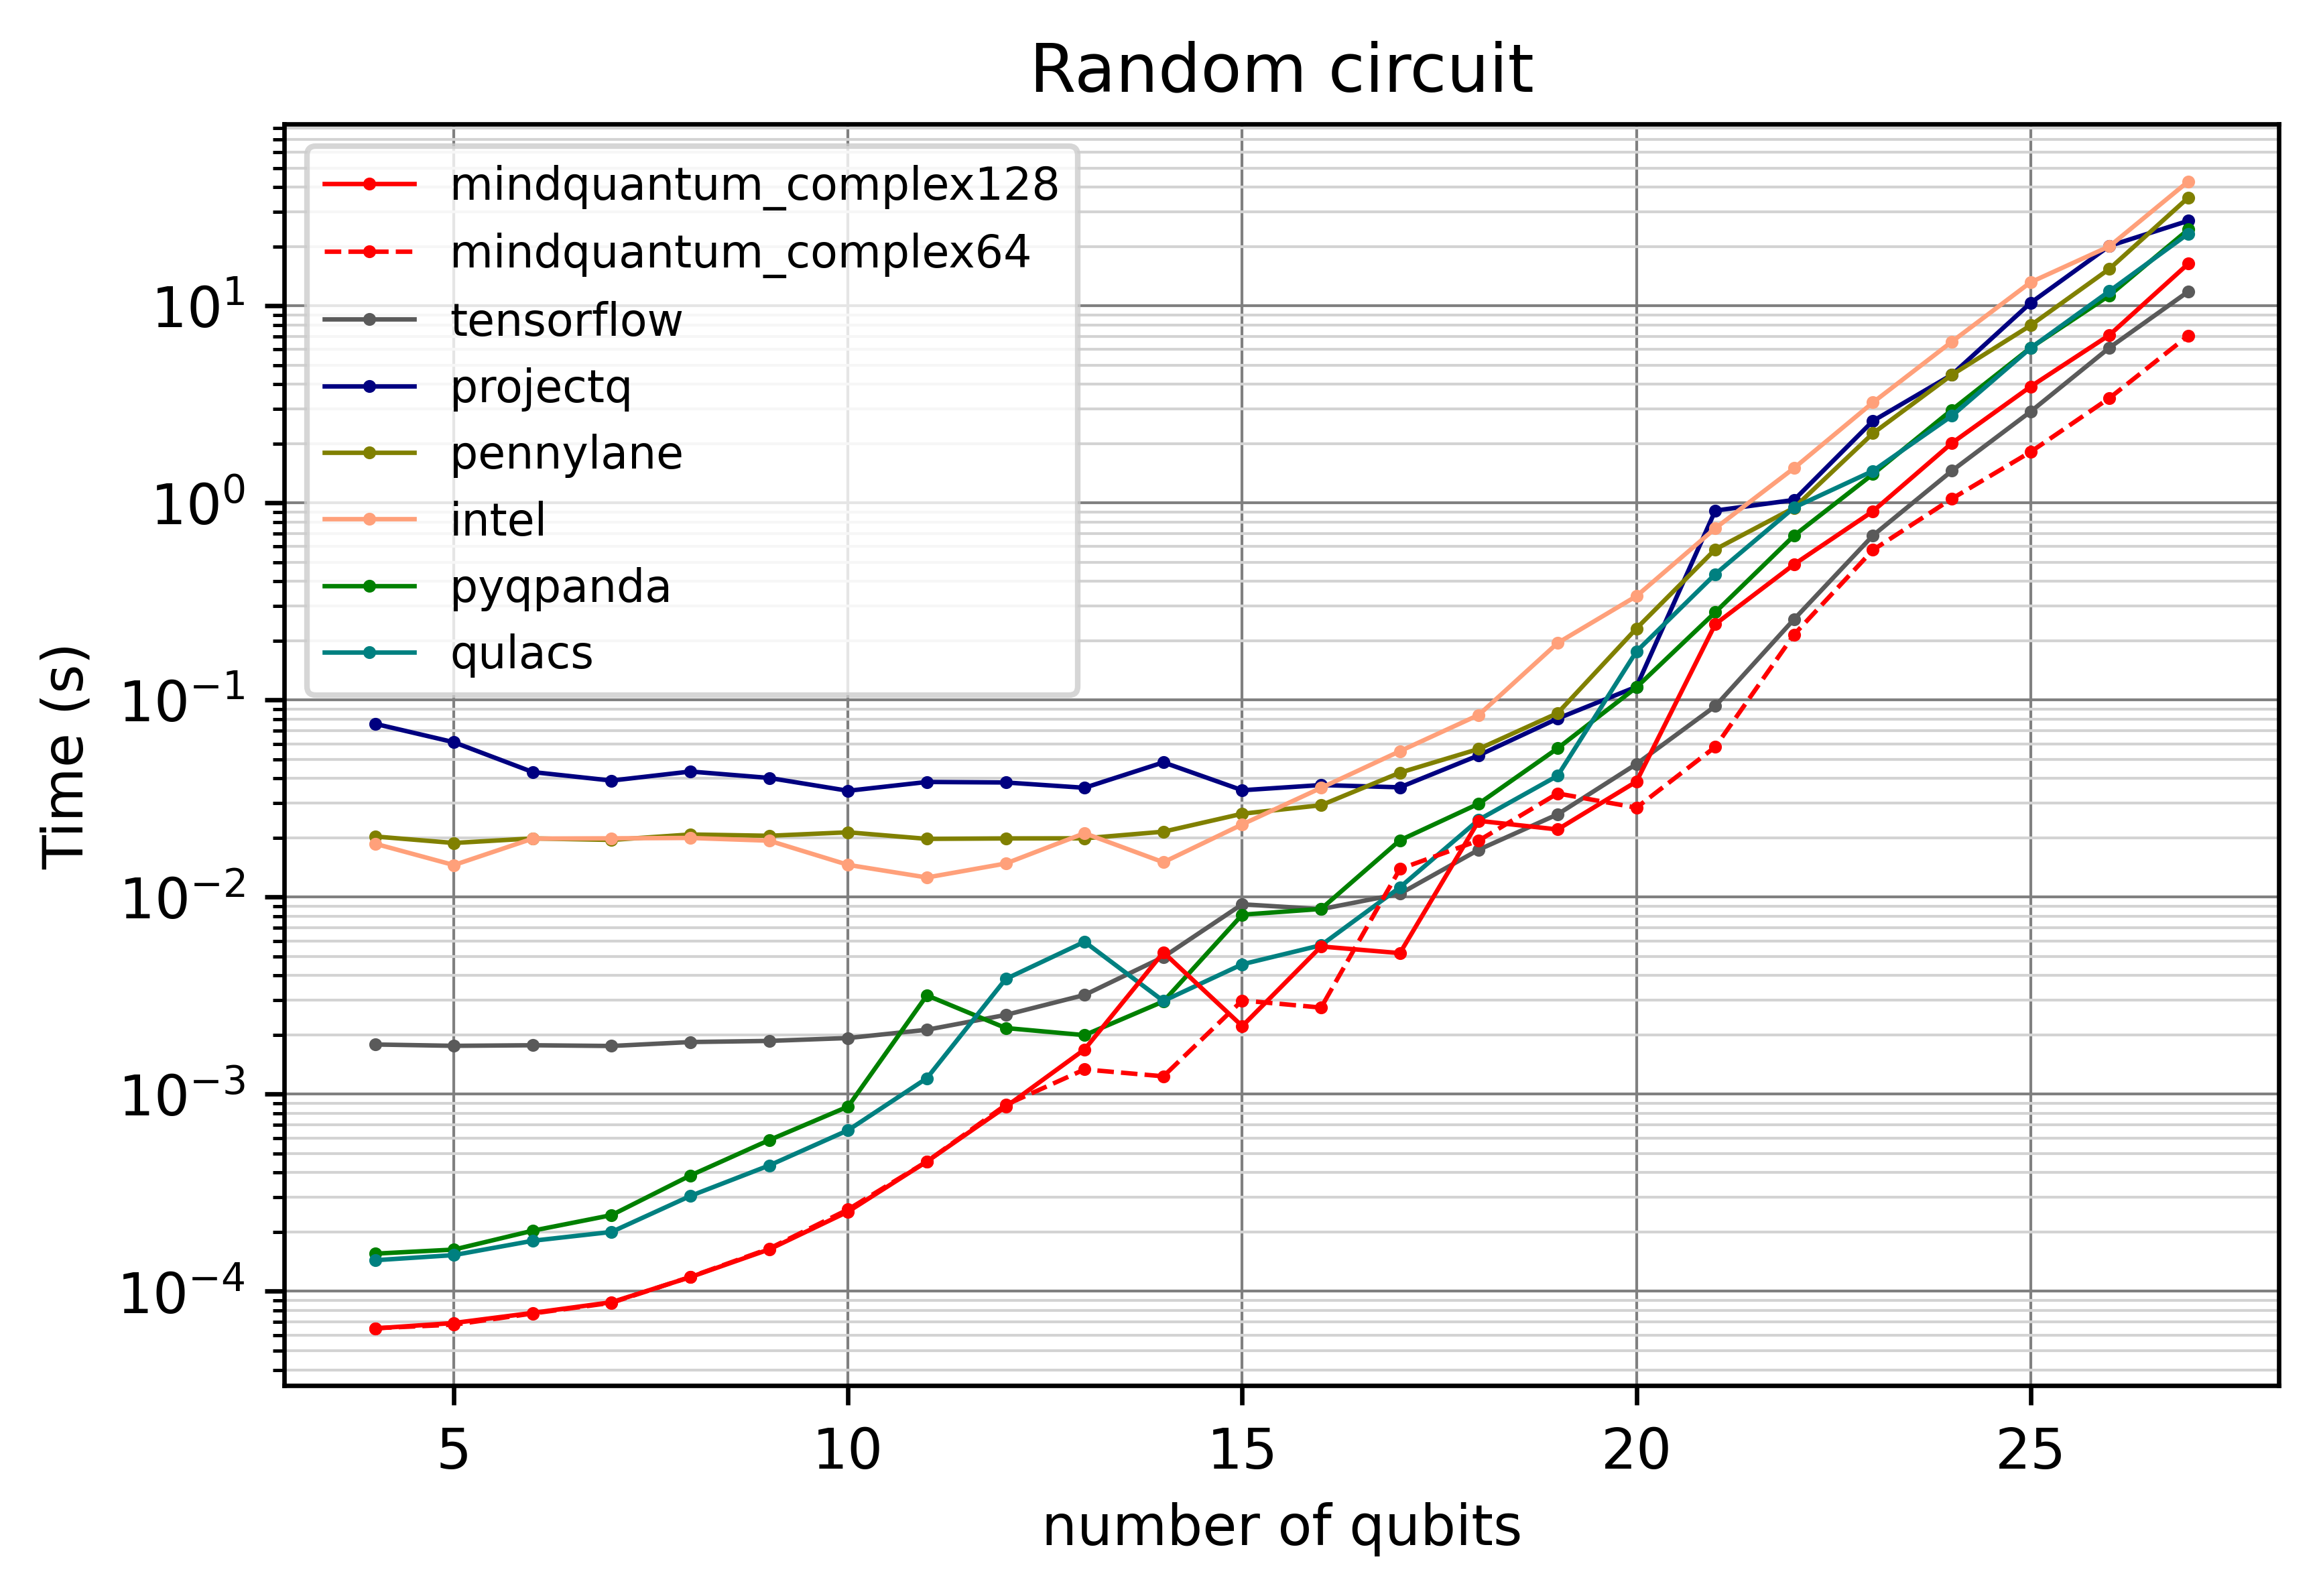
\includegraphics[width=\textwidth]{images/7_Random_circuit_CPU.png}
        \caption{Random circuit benchmark with CPU backend.}
        \label{7_random_circ_cpu}
    \end{subfigure}
    \begin{subfigure}{0.45\textwidth}
        \centering
        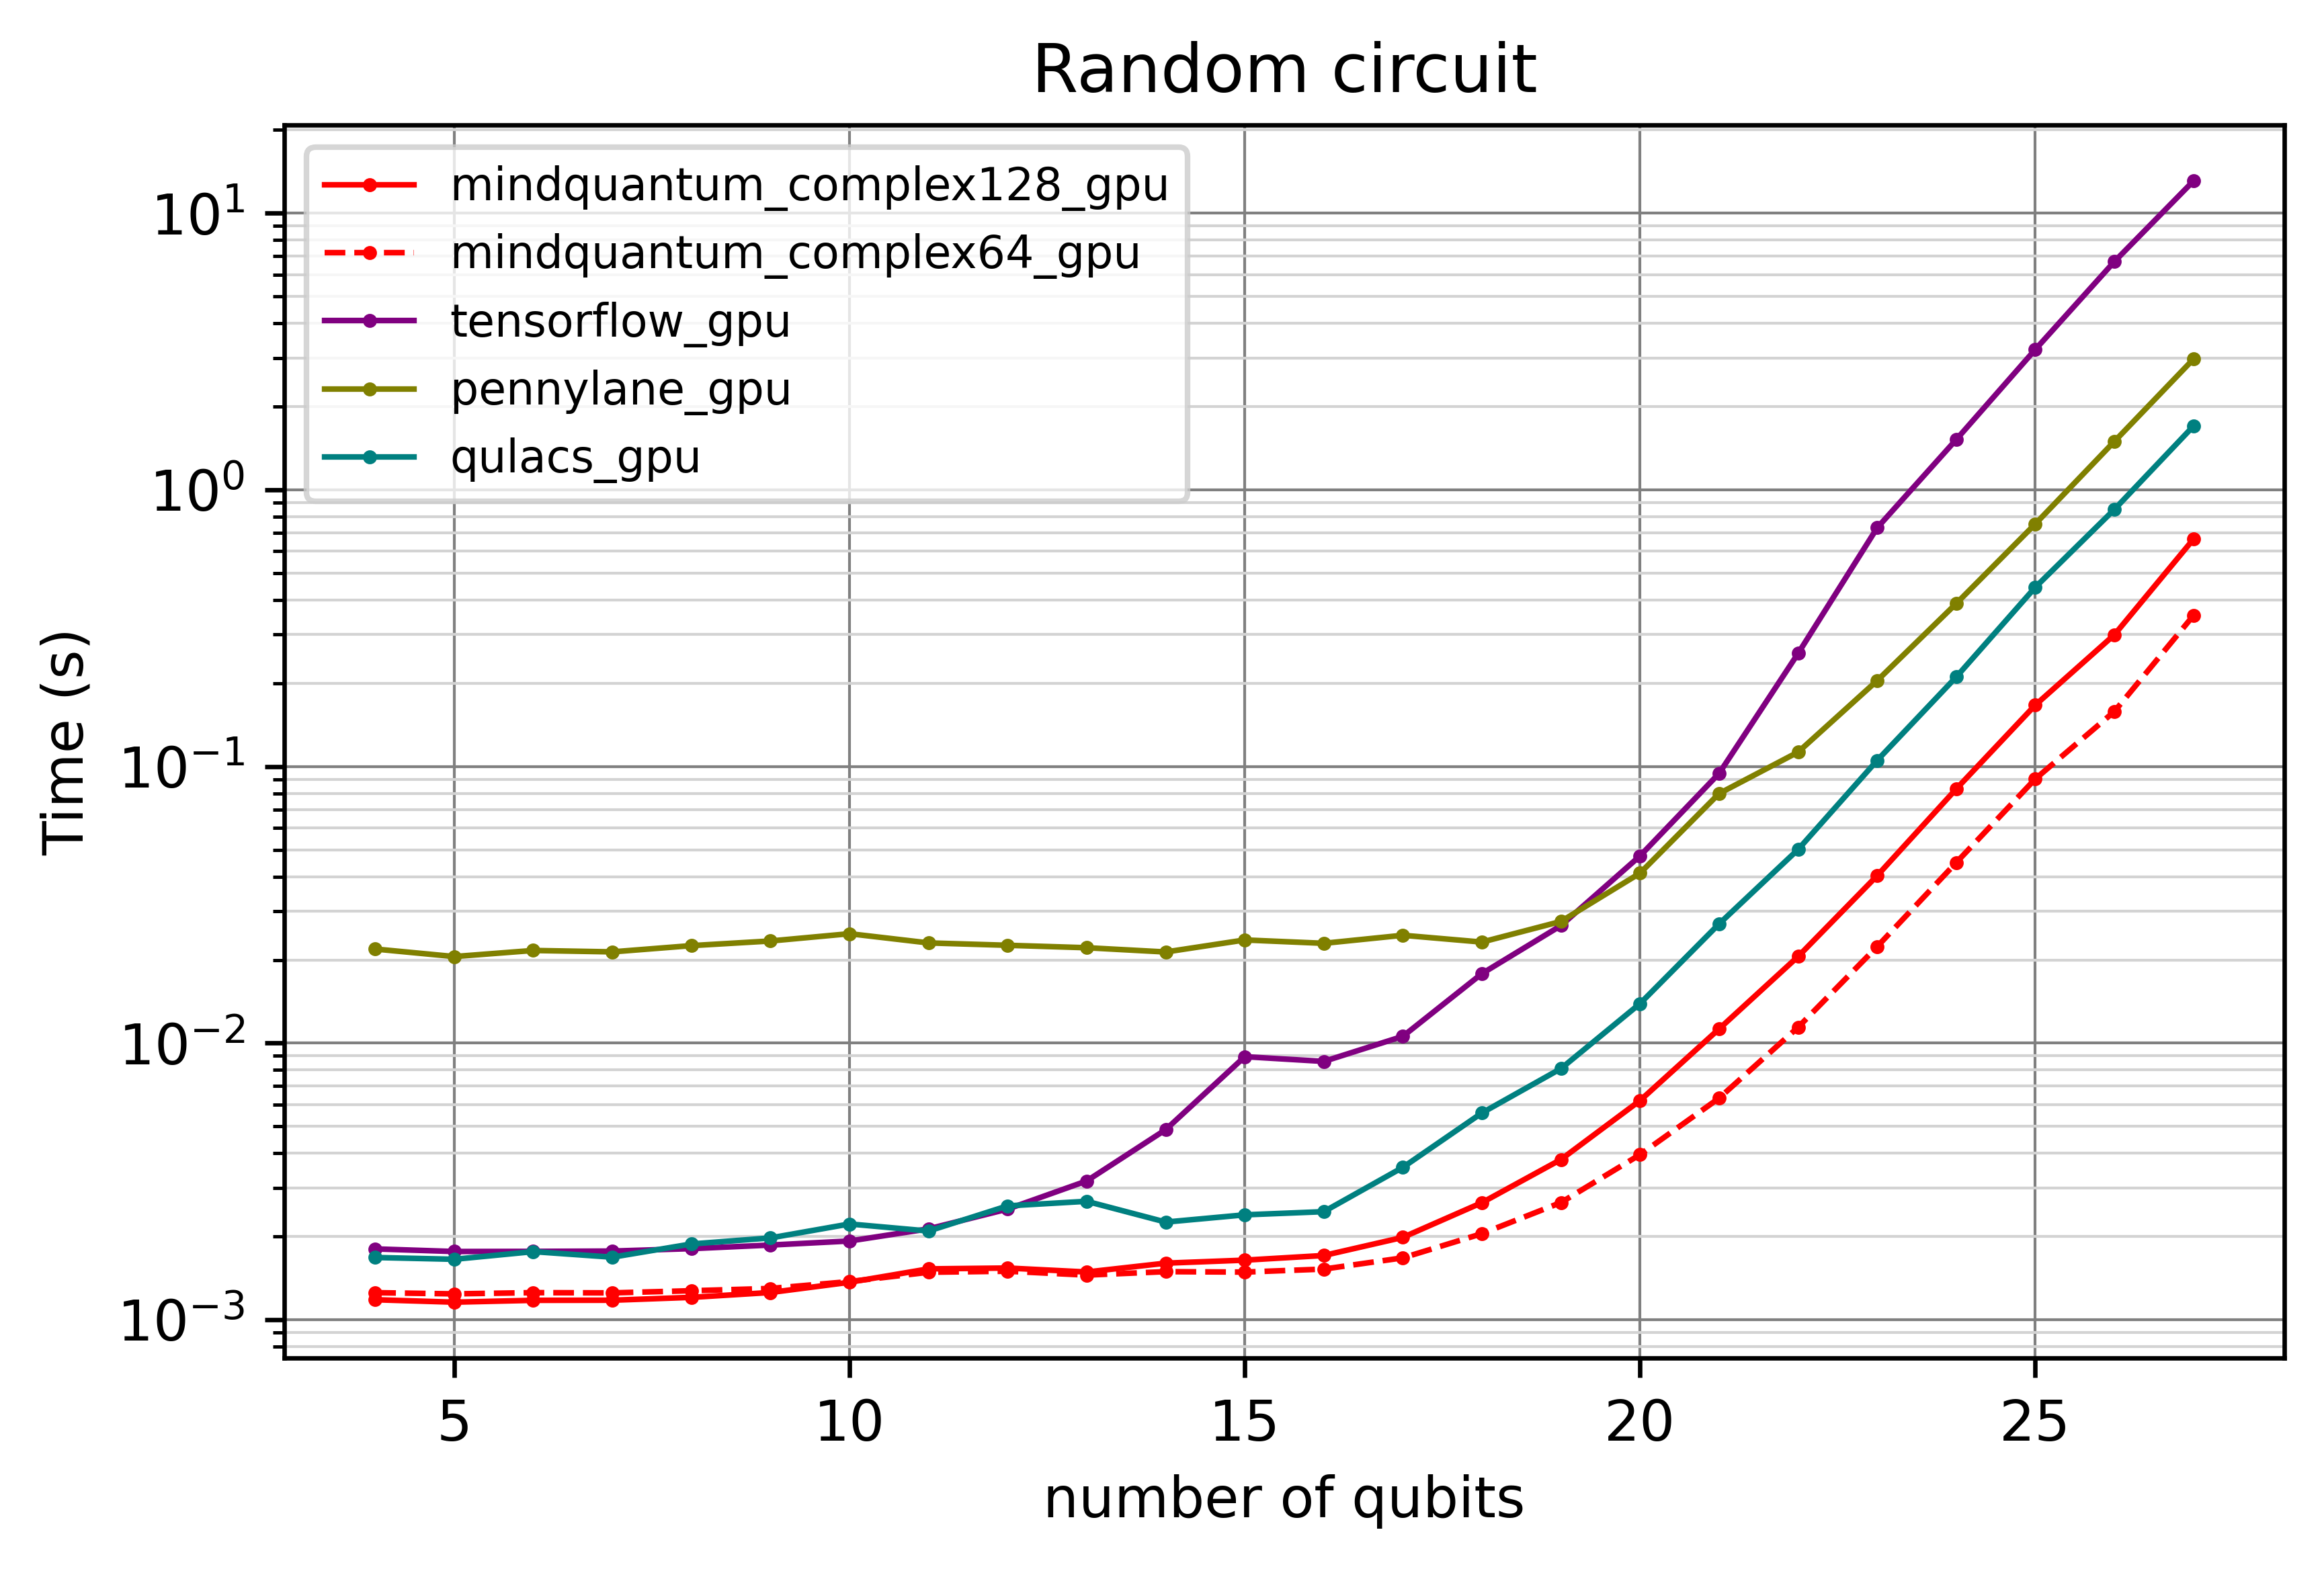
\includegraphics[width=\textwidth]{images/7_Random_circuit_GPU.png}
        \caption{Random circuit benchmark with GPU backend.}
        \label{7_random_circ_gpu}
    \end{subfigure}
    \begin{subfigure}{0.45\textwidth}
        \centering
        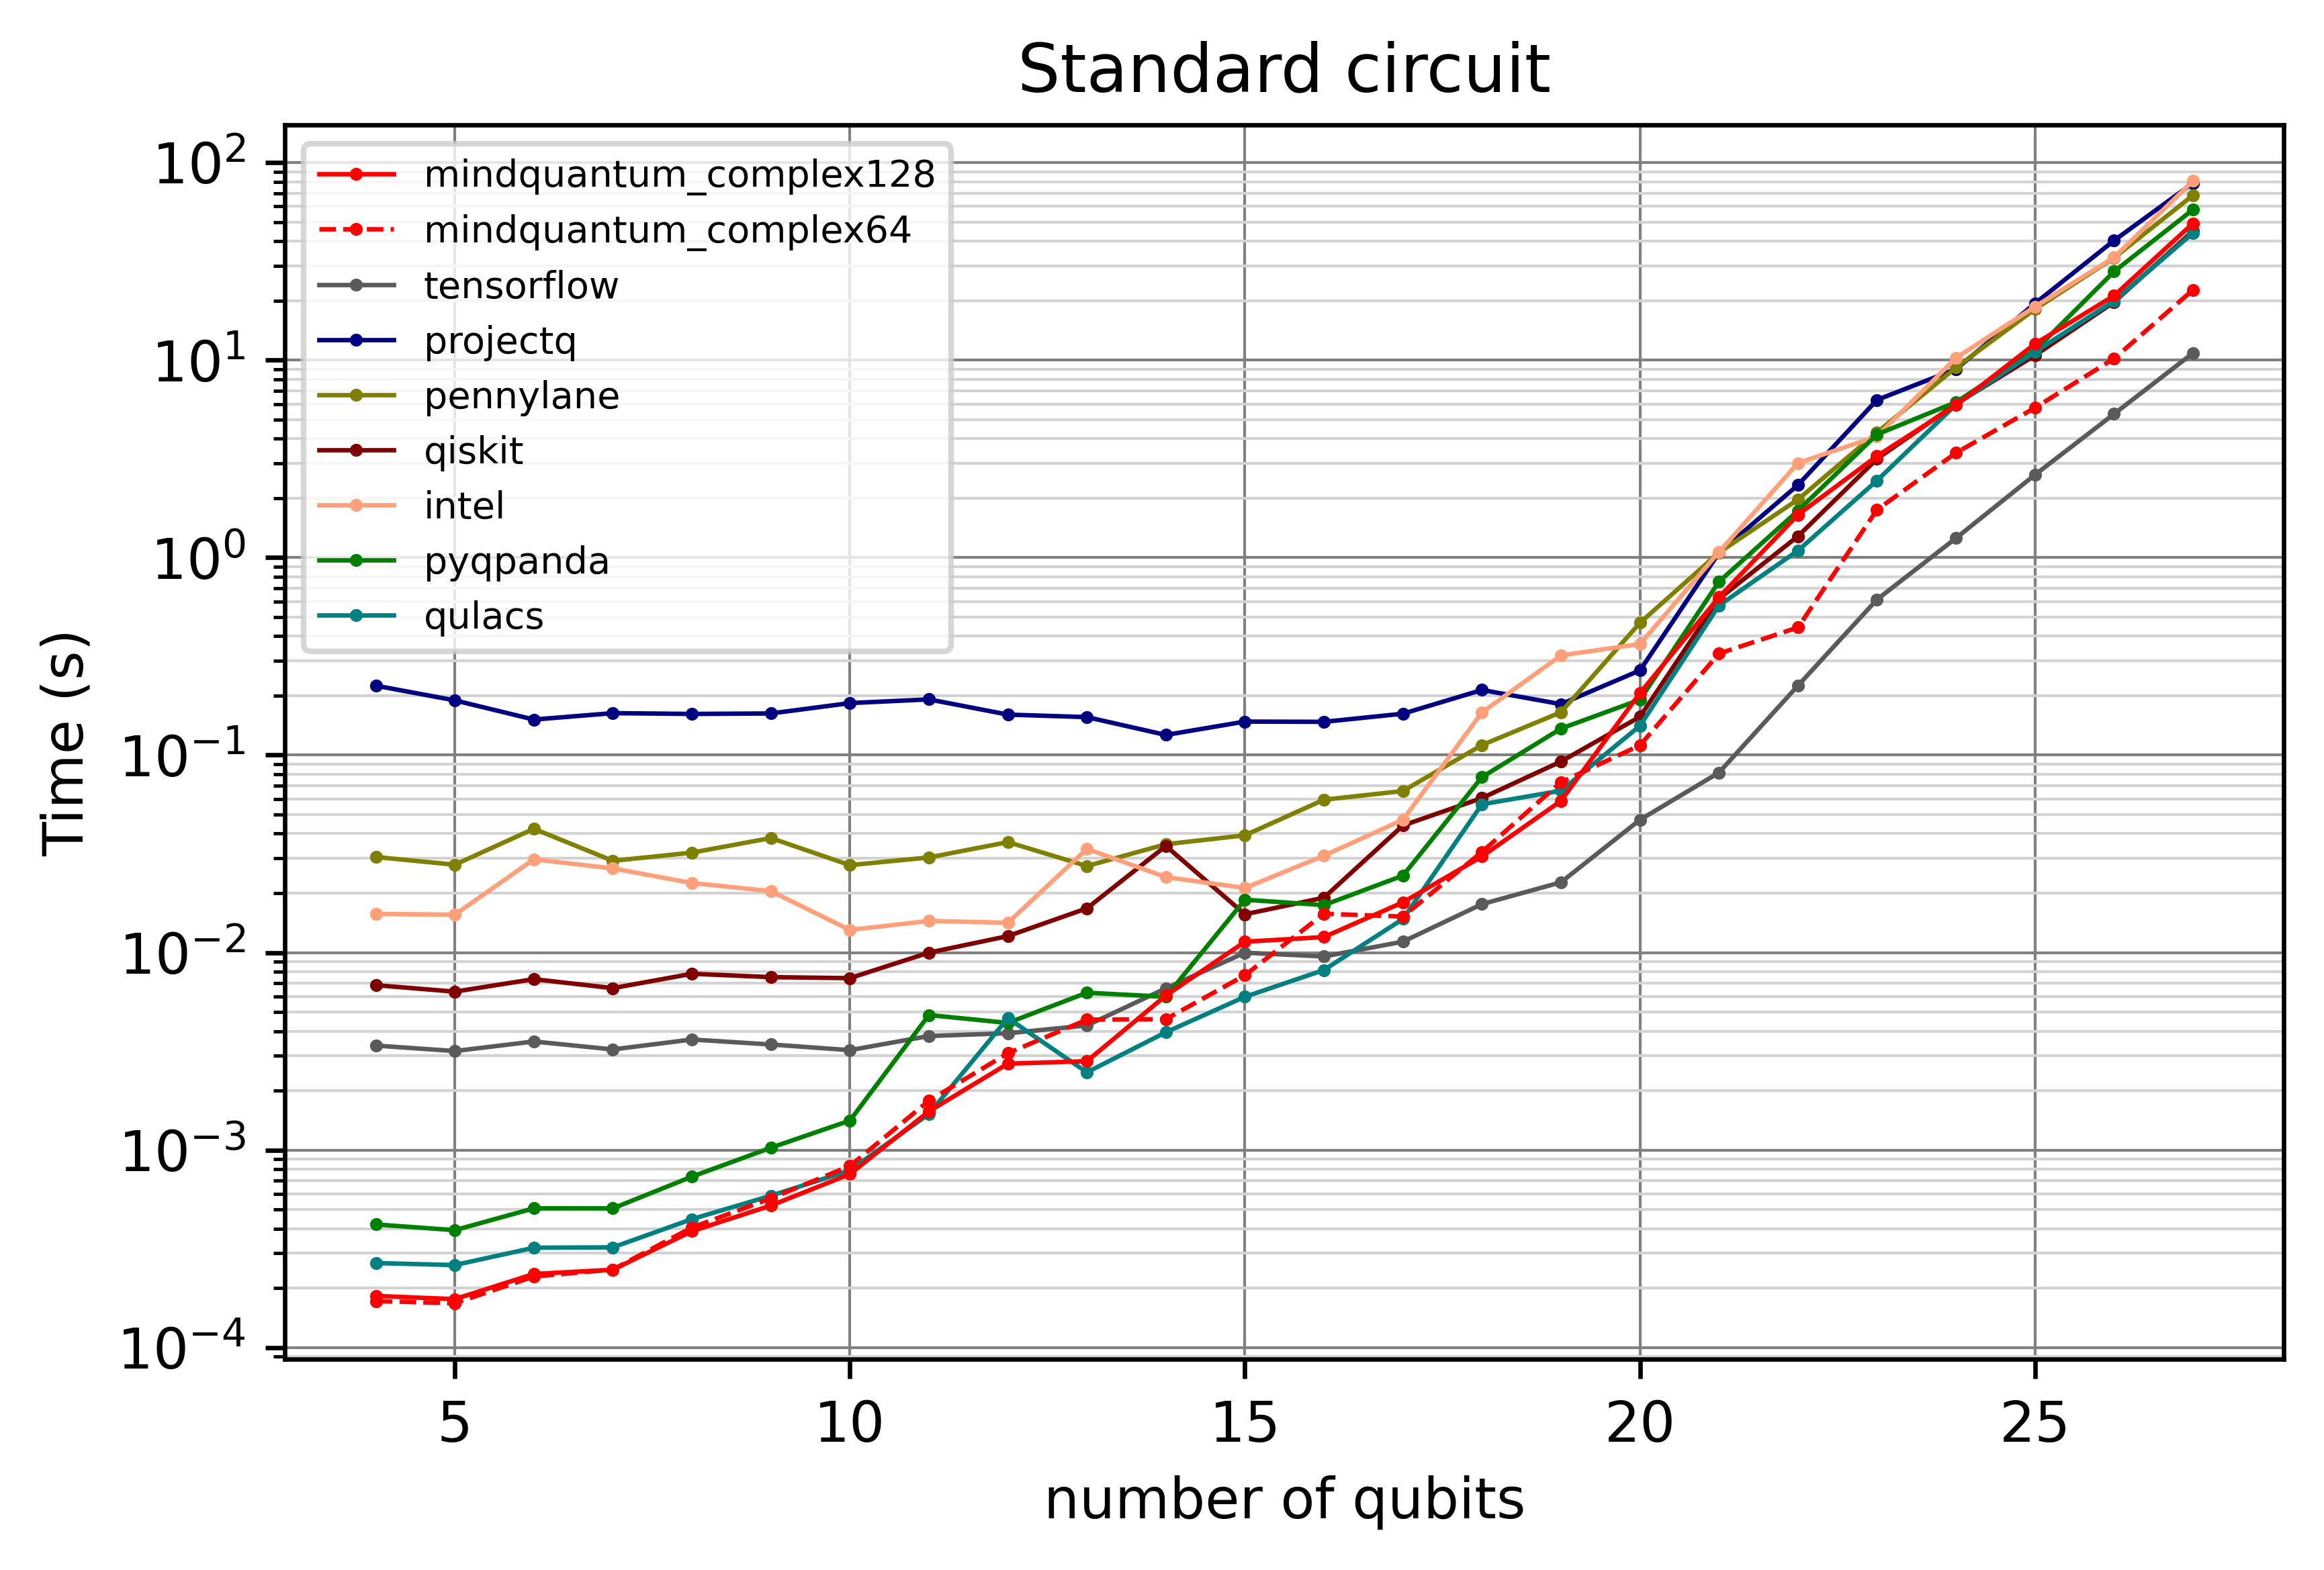
\includegraphics[width=\textwidth]{images/7_Simple_circuit_CPU.png}
        \caption{Standard circuit benchmark with CPU backend.}
        \label{7_random_circ_cpu}
    \end{subfigure}
    \begin{subfigure}{0.45\textwidth}
        \centering
        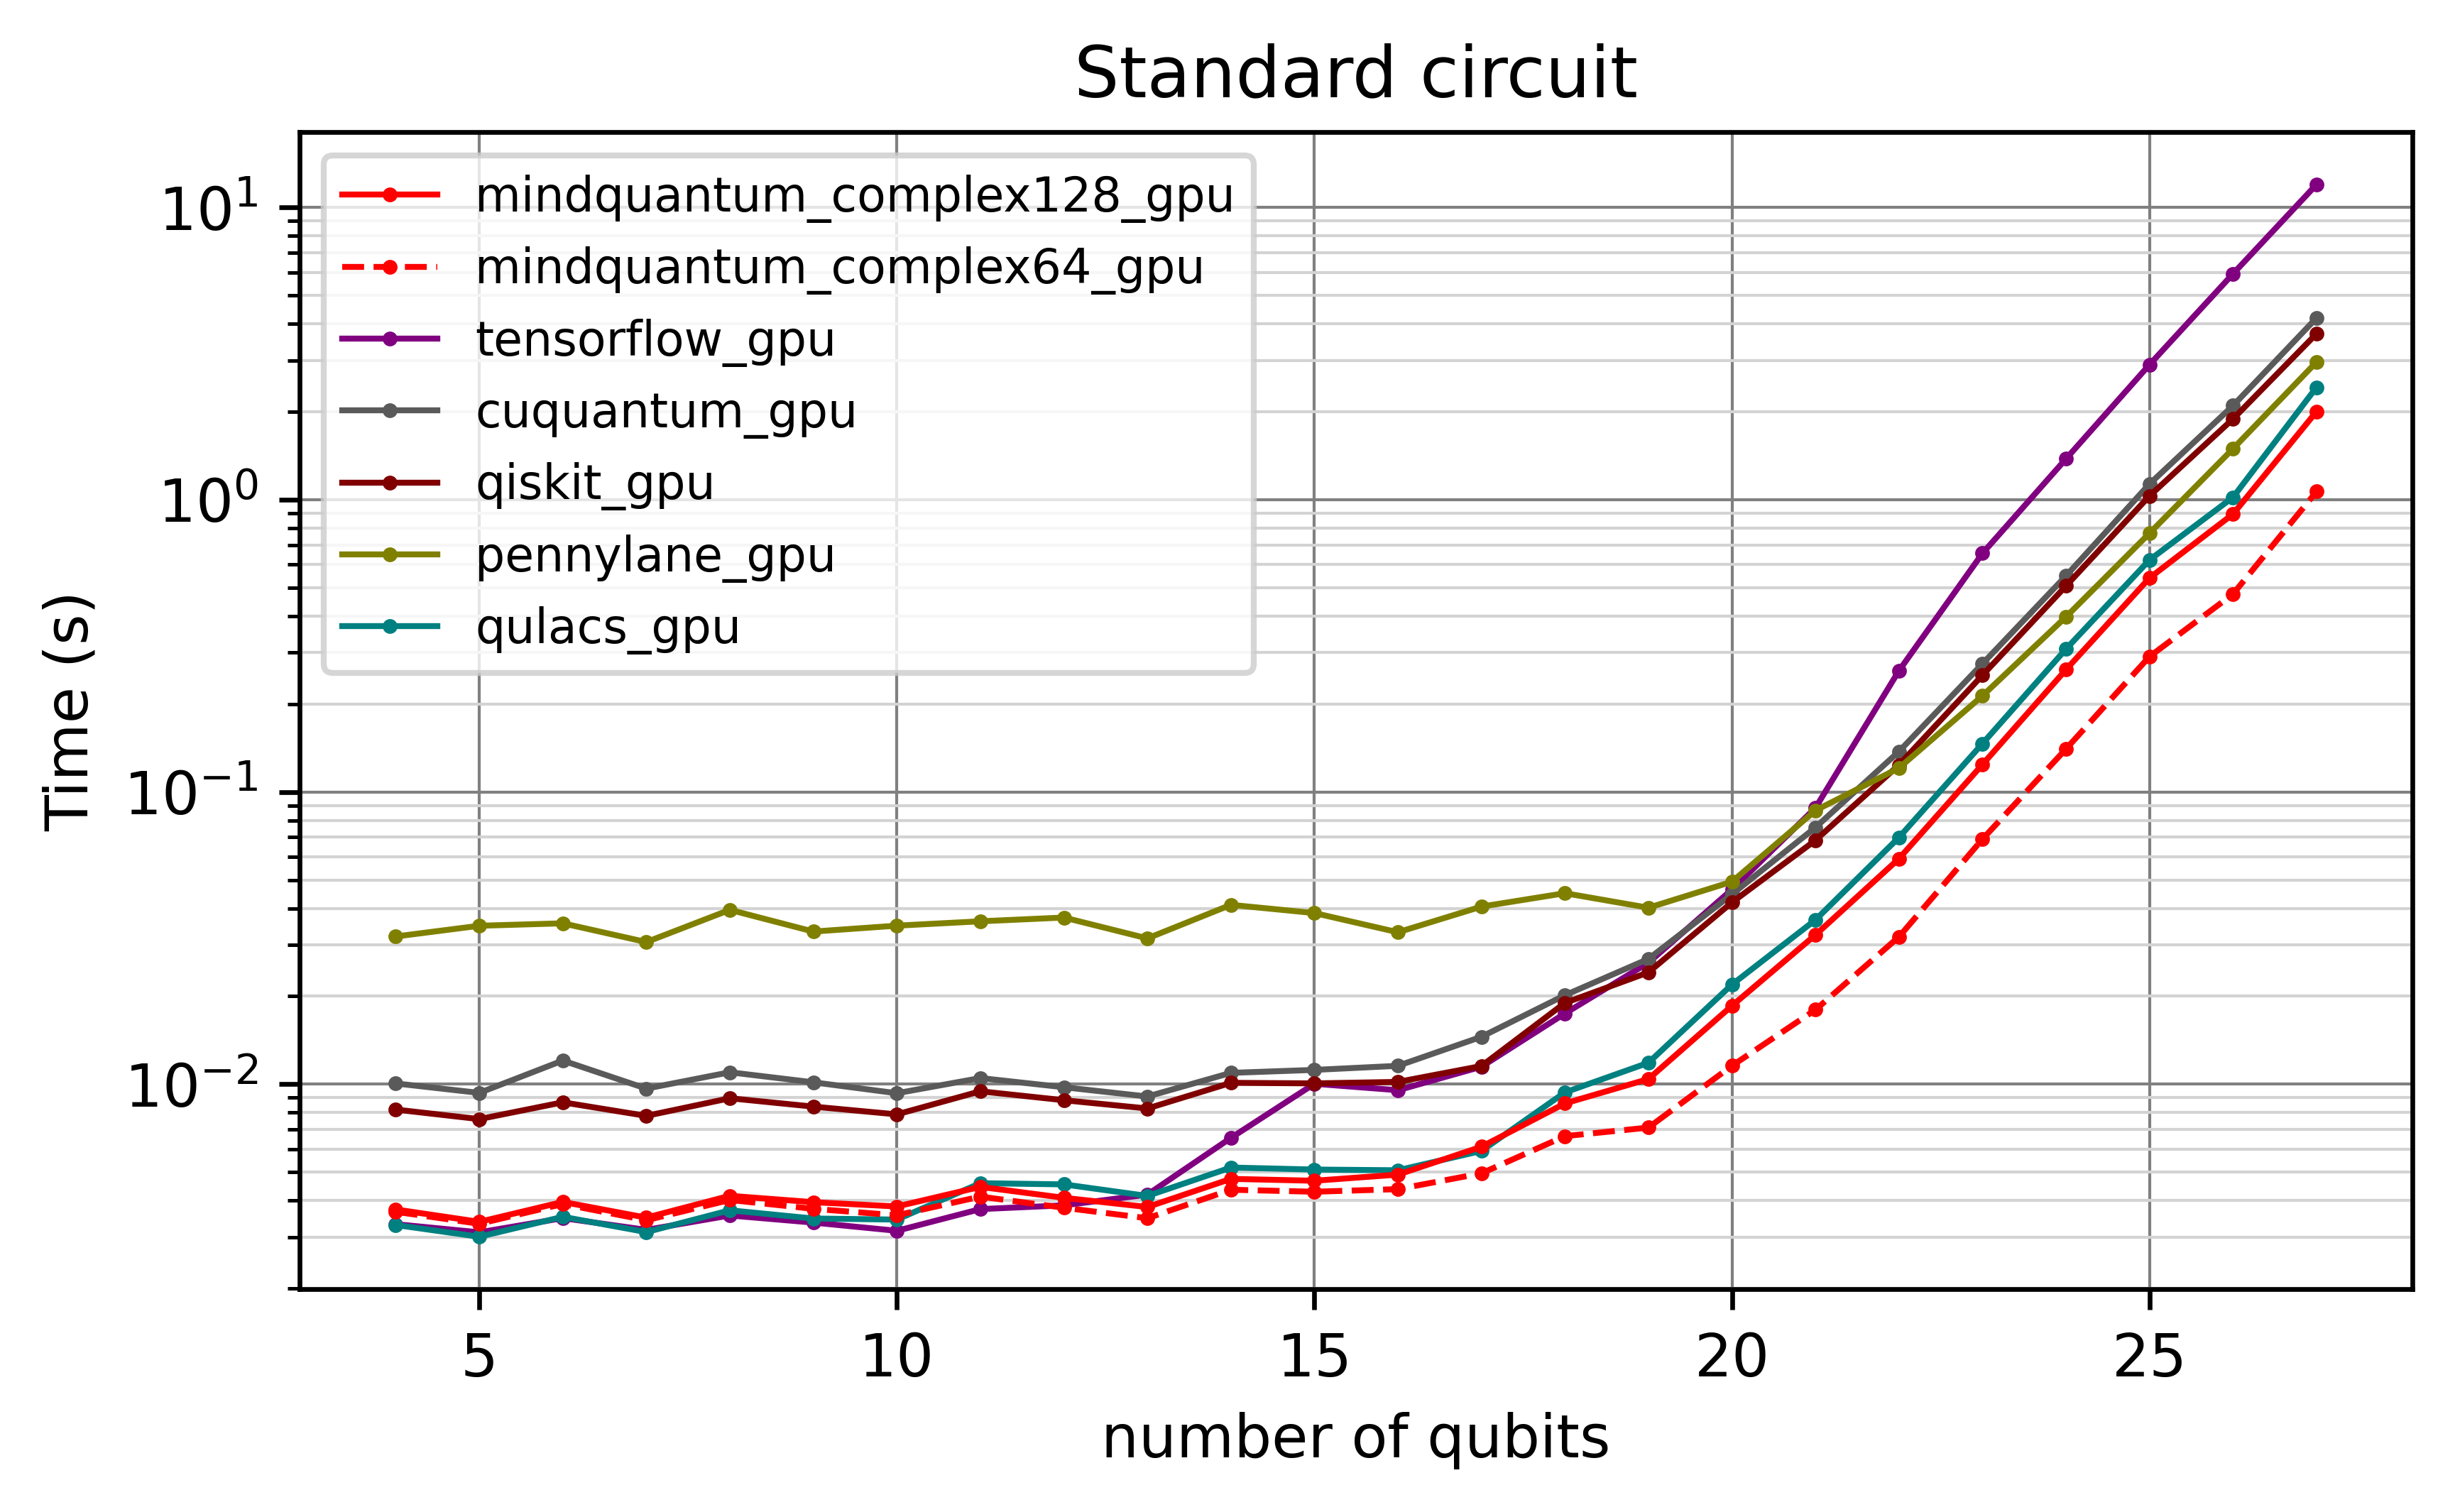
\includegraphics[width=\textwidth]{images/7_Simple_circuit_GPU.png}
        \caption{Standard circuit benchmark with GPU backend.}
        \label{7_random_circ_gpu}
    \end{subfigure}
    \caption{Benchmarking of randomly complex circuit and randomly simple circuit with different backends.}
    \label{fig:benchmark_circ}
\end{figure*}

\subsection{Running Random Circuit Task}

In random circuit benchmarking, we choose two different kinds of circuit. The first task is complex random circuit with qubit number start from 4 to 27. The complex random circuit contains X, Y, Z, H, CNOT, S, T, RX, RY, RZ, Rxx, Ryy, Rzz, SWAP gate and its control version. The second task is a simple random circuit that decomposed from the corresponded complex random circuit, and it only contains basic gate sets. The precision of simulator in benchmarking is double-precision except TensorFlow Quantum. The benchmark result is shown in Fig.~\ref{fig:benchmark_circ}.


In general, the simulation time increases exponentially with the circuit scale. However, when the number of qubits is small, \MindQuantum, Qulacs and Qpanda have a clear advantage in terms of time compared to other frameworks, which is due to the overhead of API call. It is worth noting that there is a slight dip at the 13-qubit position because \MindQuantum\ uses 13 qubits as a threshold, and when the number of qubits is greater than 13, it enables OpenMP to perform multi-threaded parallel computing, otherwise single thread simulation is used. This is because we found that multi-threaded computing would reduce the running speed when the number of qubits is small. As the circuit scale continues to increase, \MindQuantum\ and Qulacs maintain a good speed advantage, which can be judged that the two frameworks have been optimized to near the limit at the low-level implementation. When dealing with simple circuit with large qubit numbers, TensorFlow Quantum demonstrates advantages. There are two reasons for this. Firstly, it utilizes single-precision computation. Secondly, it incorporates more optimizations specifically targeted at fundamental quantum gates.

\begin{figure*}
    \centering
    \begin{subfigure}{0.9\textwidth}
        \centering
        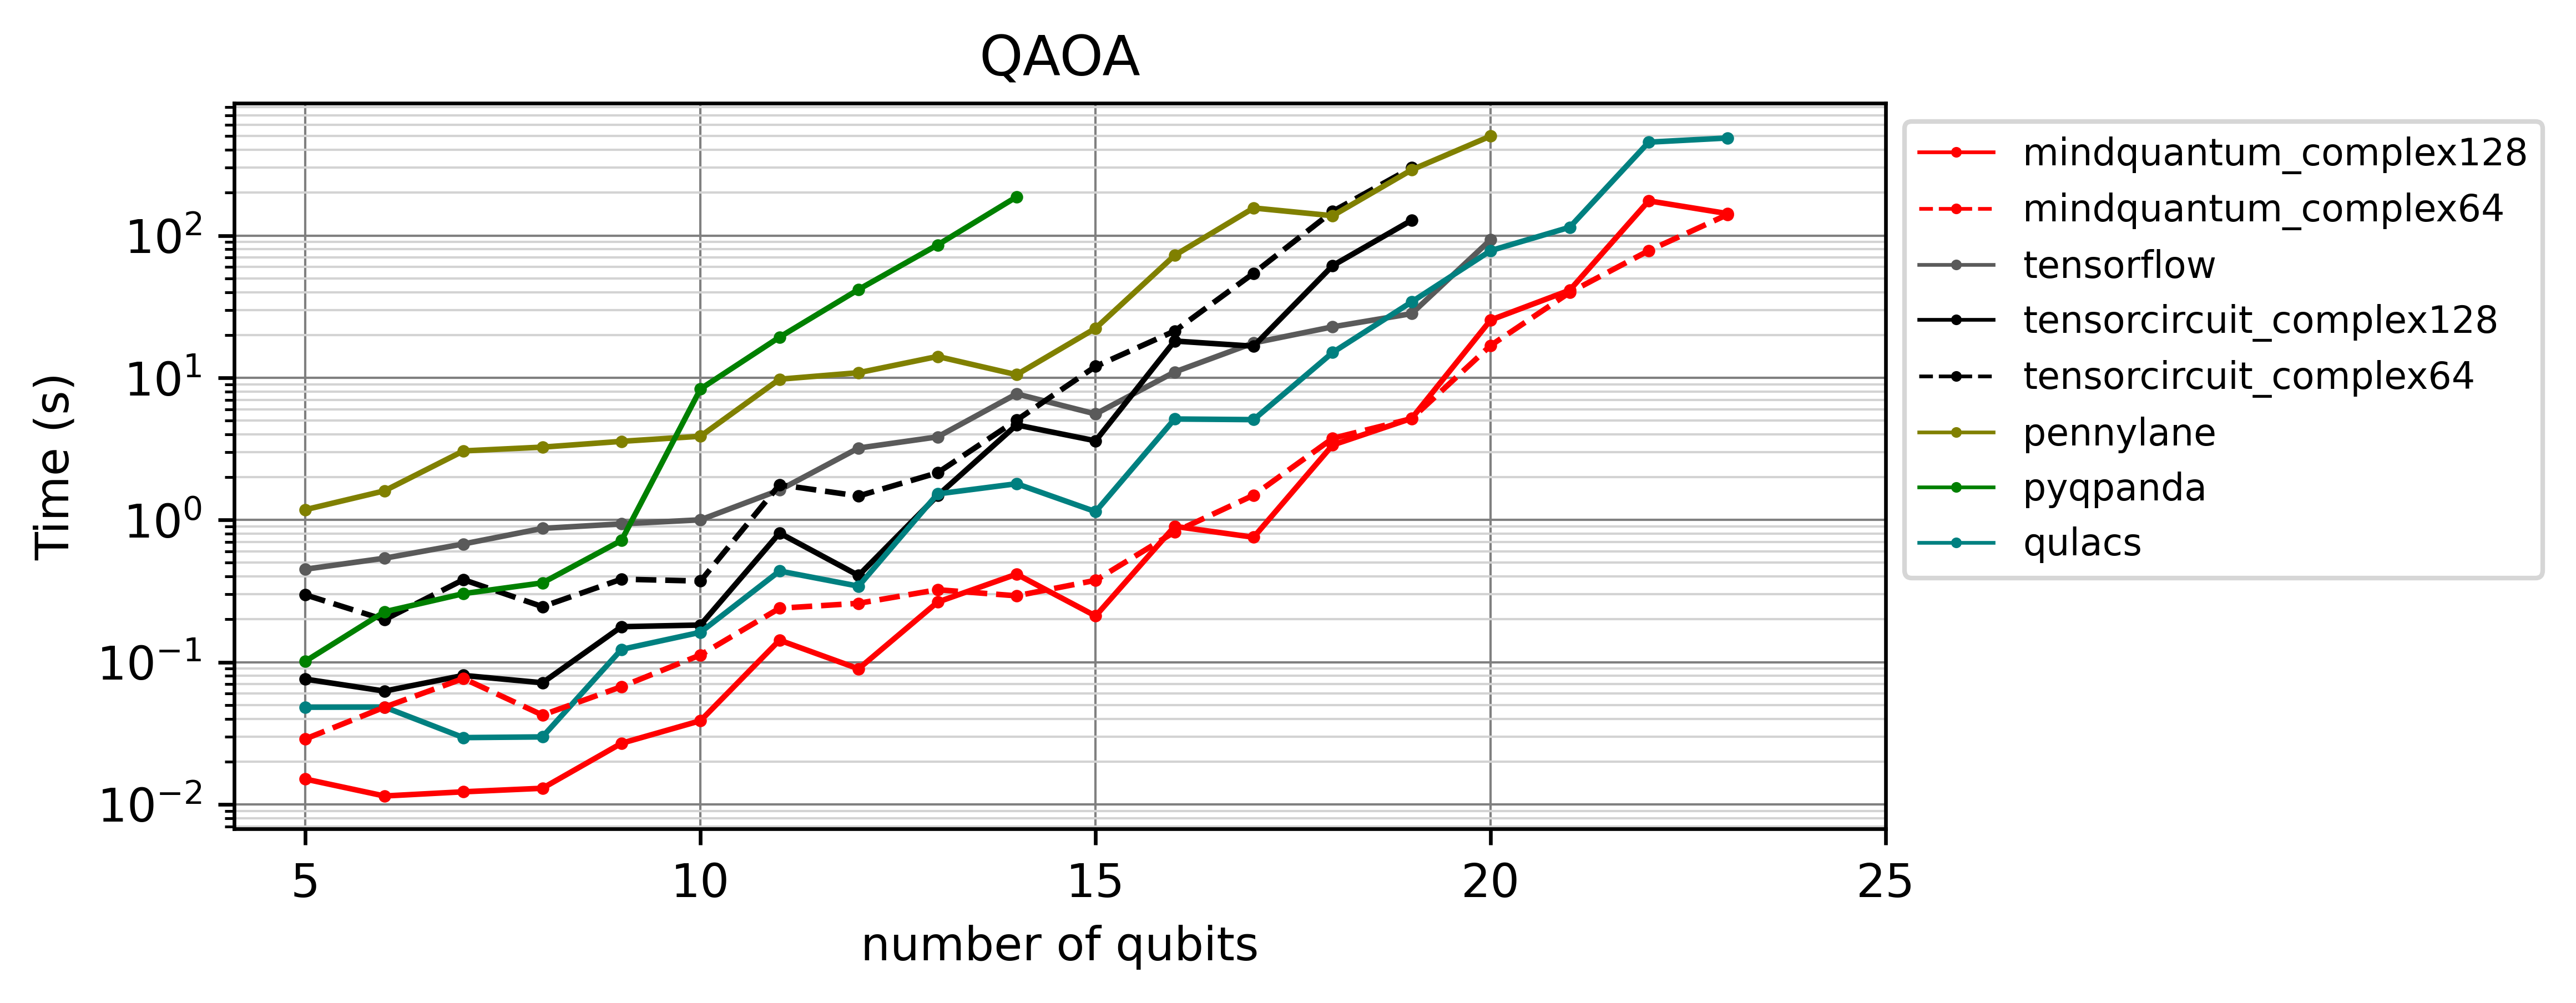
\includegraphics[width=\textwidth]{images/7_QAOA_CPU.png}
        \caption{Benchmarking of QAOA end to end optimization with regular-4 graph in CPU.}
        \label{7_regular_4_cpu}
    \end{subfigure}
    \begin{subfigure}{0.9\textwidth}
        \centering
        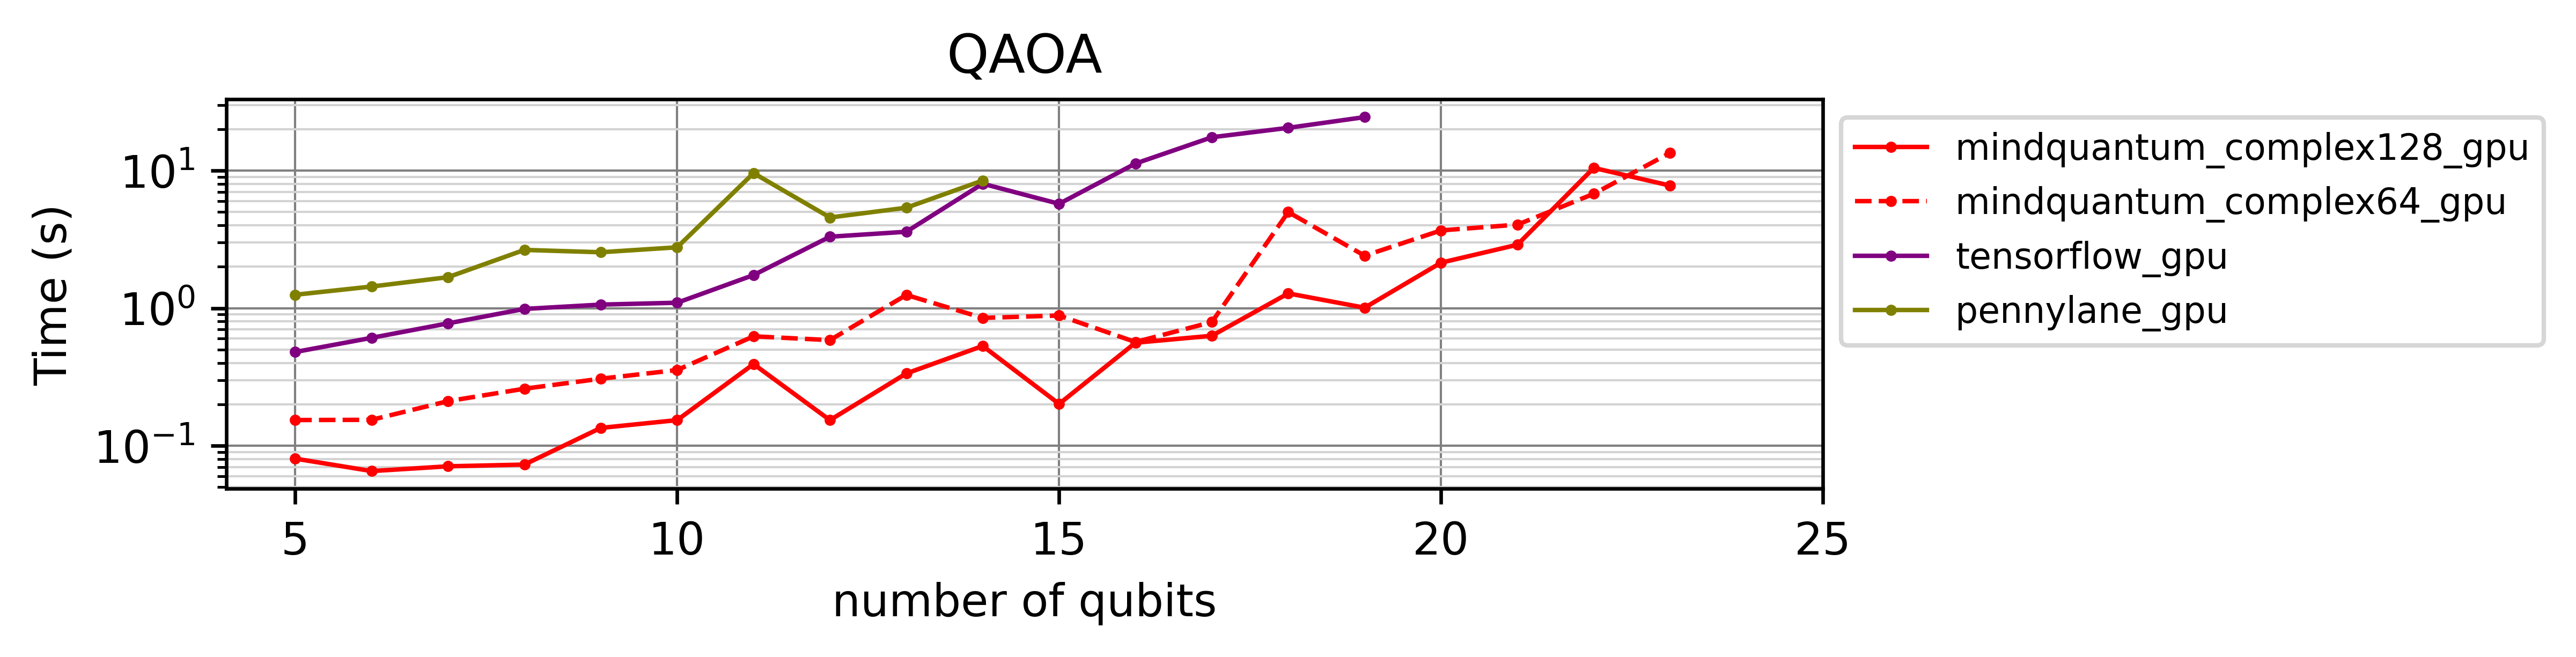
\includegraphics[width=\textwidth]{images/7_QAOA_GPU.png}
        \caption{Benchmarking of QAOA end to end optimization with regular-4 graph in GPU}
        \label{7_regular_4_gpu}
    \end{subfigure}
    \caption{Benchmarking of QAOA with different backends.}
    \label{fig:benchmark_qaoa}
\end{figure*}

\subsection{QAOA Task}

Variational quantum algorithm is also a very important algorithm in NISQ. In this part, we choose Quantum Approximate Optimization Algorithm for benchmarking, which can further demonstrate the performance of the framework in solving practical problems. We apply QAOA to solve the max-cut problem of 4-regular graphs, and the size of the problem ranges from 5 to 23 nodes. The ansatz circuit is obtained by one-step Trotter decomposition. The optimizer is \code{scipy.optimize.minimize()} with the BFGS method. Since large-scale QAOA tasks are time-consuming, we stop the execution of each framework when the running time reaches a specified threshold. Therefore, in the result images, the maximum number of qubits that each framework data point can achieve is not consistent. The benchmark result is shown in Fig.~\ref{fig:benchmark_qaoa}.

Overall, as the problem size increases, the solution time of all frameworks grows exponentially. However, \MindQuantum\ is at least one orders of magnitude faster than other frameworks for problems. This is mainly due to MindQuantum's optimized adjoint method for getting gradient parameterized quantum circuit and efficient implementation of circuit evolution.
